\documentclass[a4paper,11pt,fleqn,twoside,openright]{memoir} 	% Openright aabner kapitler paa hoejresider (openany begge)

%%%% PACKAGES %%%%

% ¤¤ Oversaettelse og tegnsaetning ¤¤ %
\usepackage[utf8]{inputenc}					% Input-indkodning af tegnsaet (UTF8)
\usepackage[english]{babel}					% Dokumentets sprog
\usepackage[T1]{fontenc}					% Output-indkodning af tegnsaet (T1)
\usepackage{ragged2e,anyfontsize}			% Justering af elementer
\usepackage{fixltx2e}						% Retter forskellige fejl i LaTeX-kernen
																			
% ¤¤ Figurer og tabeller (floats) ¤¤ %
\usepackage{graphicx} 						% Haandtering af eksterne billeder (JPG, PNG, PDF)
\usepackage{multirow}                		% Fletning af raekker og kolonner (\multicolumn og \multirow)
\usepackage{colortbl} 						% Farver i tabeller (fx \columncolor, \rowcolor og \cellcolor)
\usepackage[dvipsnames]{xcolor}				% Definer farver med \definecolor. Se mere: http://en.wikibooks.org/wiki/LaTeX/Colors
\usepackage{flafter}						% Soerger for at floats ikke optraeder i teksten foer deres reference
\let\newfloat\relax 						% Justering mellem float-pakken og memoir
\usepackage{float}							% Muliggoer eksakt placering af floats, f.eks. \begin{figure}[H]
%\usepackage{eso-pic}						% Tilfoej billedekommandoer paa hver side
%\usepackage{wrapfig}						% Indsaettelse af figurer omsvoebt af tekst. \begin{wrapfigure}{Placering}{Stoerrelse}
%\usepackage{multicol}         	        	% Muliggoer tekst i spalter
%\usepackage{rotating}						% Rotation af tekst med \begin{sideways}...\end{sideways}
\usepackage{array}


% ¤¤ Matematik mm. ¤¤
\usepackage{amsmath,amssymb,stmaryrd} 		% Avancerede matematik-udvidelser
\usepackage{mathtools}						% Andre matematik- og tegnudvidelser
\usepackage{textcomp}                 		% Symbol-udvidelser (f.eks. promille-tegn med \textperthousand )
\usepackage{siunitx}						% Flot og konsistent praesentation af tal og enheder med \si{enhed} og \SI{tal}{enhed}
\sisetup{output-decimal-marker = {,}}		% Opsaetning af \SI (DE for komma som decimalseparator) 
\usepackage[version=3]{mhchem} 				% Kemi-pakke til flot og let notation af formler, f.eks. \ce{Fe2O3}
%\usepackage{rsphrase}						% Kemi-pakke til RS-saetninger, f.eks. \rsphrase{R1}

% ¤¤ Referencer og kilder ¤¤ %
\usepackage[danish]{varioref}				% Muliggoer bl.a. krydshenvisninger med sidetal (\vref)
\usepackage{natbib}							% Udvidelse med naturvidenskabelige citationsmodeller
%\usepackage{xr}							% Referencer til eksternt dokument med \externaldocument{<NAVN>}
%\usepackage{glossaries}					% Terminologi- eller symbolliste (se mere i Daleifs Latex-bog)

% ¤¤ Misc. ¤¤ %
\usepackage{listings}						% Placer kildekode i dokumentet med \begin{lstlisting}...\end{lstlisting}
\usepackage{lipsum}							% Dummy text \lipsum[..]
\usepackage[shortlabels]{enumitem}			% Muliggoer enkelt konfiguration af lister
\usepackage{pdfpages}						% Goer det muligt at inkludere pdf-dokumenter med kommandoen \includepdf[pages={x-y}]{fil.pdf}	
\pdfoptionpdfminorversion=6					% Muliggoer inkludering af pdf dokumenter, af version 1.6 og hoejere
\pretolerance=2500 							% Justering af afstand mellem ord (hoejt tal, mindre orddeling og mere luft mellem ord)

% Kommentarer og rettelser med \fxnote. Med 'final' i stedet for 'draft' udloeser hver note en error i den faerdige rapport.
\usepackage[footnote,draft,danish,silent,nomargin]{fixme}		

\usepackage{todonotes}

\usepackage{lastpage}

%%%% CUSTOM SETTINGS %%%%

% ¤¤ Marginer ¤¤ %
\setlrmarginsandblock{3.5cm}{2.5cm}{*}		% \setlrmarginsandblock{Indbinding}{Kant}{Ratio}
\setulmarginsandblock{2.5cm}{3.0cm}{*}		% \setulmarginsandblock{Top}{Bund}{Ratio}
\checkandfixthelayout 						% Oversaetter vaerdier til brug for andre pakker

%	¤¤ Afsnitsformatering ¤¤ %
\setlength{\parindent}{0mm}           		% Stoerrelse af indryk
\setlength{\parskip}{3mm}          			% Afstand mellem afsnit ved brug af double Enter
\linespread{1,1}							% Linie afstand

% ¤¤ Litteraturlisten ¤¤ %
\bibpunct[,]{[}{]}{;}{a}{,}{,} 				% Definerer de 6 parametre ved Harvard henvisning (bl.a. parantestype og seperatortegn)
\bibliographystyle{bibtex/harvard}			% Udseende af litteraturlisten.

% ¤¤ Indholdsfortegnelse ¤¤ %
\setsecnumdepth{subsection}		 			% Dybden af nummerede overkrifter (part/chapter/section/subsection)
\maxsecnumdepth{subsection}					% Dokumentklassens graense for nummereringsdybde
\settocdepth{subsection} 					% Dybden af indholdsfortegnelsen

% ¤¤ Lister ¤¤ %
\setlist{
  topsep=0pt,								% Vertikal afstand mellem tekst og listen
  itemsep=-1ex,								% Vertikal afstand mellem items
} 

% ¤¤ Visuelle referencer ¤¤ %
\usepackage[colorlinks]{hyperref}			% Danner klikbare referencer (hyperlinks) i dokumentet.
\hypersetup{colorlinks = true,				% Opsaetning af farvede hyperlinks (interne links, citeringer og URL)
    linkcolor = black,
    citecolor = black,
    urlcolor = black
}

% ¤¤ Opsaetning af figur- og tabeltekst ¤¤ %
\captionnamefont{\small\bfseries\itshape}	% Opsaetning af tekstdelen ('Figur' eller 'Tabel')
\captiontitlefont{\small}					% Opsaetning af nummerering
\captiondelim{. }							% Seperator mellem nummerering og figurtekst
\hangcaption								% Venstrejusterer flere-liniers figurtekst under hinanden
\captionwidth{\linewidth}					% Bredden af figurteksten
\setlength{\belowcaptionskip}{0pt}			% Afstand under figurteksten
		
% ¤¤ Opsaetning af listings ¤¤ %
\definecolor{commentGreen}{RGB}{34,139,24}
\definecolor{stringPurple}{RGB}{208,76,239}

\lstset{language=Matlab,					% Sprog
	basicstyle=\ttfamily\scriptsize,		% Opsaetning af teksten
	keywords={for,if,while,else,elseif,		% Noegleord at fremhaeve
			  end,break,return,case,
			  switch,function},
	keywordstyle=\color{blue},				% Opsaetning af noegleord
	commentstyle=\color{commentGreen},		% Opsaetning af kommentarer
	stringstyle=\color{stringPurple},		% Opsaetning af strenge
	showstringspaces=false,					% Mellemrum i strenge enten vist eller blanke
	numbers=left, numberstyle=\tiny,		% Linjenumre
	extendedchars=true, 					% Tillader specielle karakterer
	columns=flexible,						% Kolonnejustering
	breaklines, breakatwhitespace=true,		% Bryd lange linjer
}

% ¤¤ Navngivning ¤¤ %
%\addto\captionsdanish{
%	\renewcommand\appendixname{Appendiks}
%	\renewcommand\contentsname{Indholdsfortegnelse}	
%	\renewcommand\appendixpagename{Appendiks}
%	\renewcommand\appendixtocname{Appendiks}
%	\renewcommand\cftchaptername{\chaptername~}				% Skriver "Kapitel" foran kapitlerne i indholdsfortegnelsen
%	\renewcommand\cftappendixname{\appendixname~}			% Skriver "Appendiks" foran appendiks i indholdsfortegnelsen
%	}

% ¤¤ Kapiteludssende ¤¤ %
\definecolor{numbercolor}{gray}{0.7}		% Definerer en farve til brug til kapiteludseende
\newif\ifchapternonum

\makechapterstyle{jenor}{					% Definerer kapiteludseende frem til ...
  \renewcommand\beforechapskip{0pt}
  \renewcommand\printchaptername{}
  \renewcommand\printchapternum{}
  \renewcommand\printchapternonum{\chapternonumtrue}
  \renewcommand\chaptitlefont{\fontfamily{pbk}\fontseries{db}\fontshape{n}\fontsize{25}{35}\selectfont\raggedleft}
  \renewcommand\chapnumfont{\fontfamily{pbk}\fontseries{m}\fontshape{n}\fontsize{1in}{0in}\selectfont\color{numbercolor}}
  \renewcommand\printchaptertitle[1]{%
    \noindent
    \ifchapternonum
    \begin{tabularx}{\textwidth}{X}
    {\let\\\newline\chaptitlefont ##1\par} 
    \end{tabularx}
    \par\vskip-2.5mm\hrule
    \else
    \begin{tabularx}{\textwidth}{Xl}
    {\parbox[b]{\linewidth}{\chaptitlefont ##1}} & \raisebox{-15pt}{\chapnumfont \thechapter}
    \end{tabularx}
    \par\vskip2mm\hrule
    \fi
  }
}											% ... her

\chapterstyle{jenor}						% Valg af kapiteludseende - Google 'memoir chapter styles' for alternativer

% ¤¤ Sidehoved ¤¤ %

\makepagestyle{Uni}							% Definerer sidehoved og sidefod udseende frem til ...
\makepsmarks{Uni}{%
	\createmark{chapter}{left}{shownumber}{}{. \ }
	\createmark{section}{right}{shownumber}{}{. \ }
	\createplainmark{toc}{both}{\contentsname}
	\createplainmark{lof}{both}{\listfigurename}
	\createplainmark{lot}{both}{\listtablename}
	\createplainmark{bib}{both}{\bibname}
	\createplainmark{index}{both}{\indexname}
	\createplainmark{glossary}{both}{\glossaryname}
}
\nouppercaseheads											% Ingen Caps oenskes

\makeevenhead{Uni}{Gruppe B131}{}{\leftmark}				% Definerer lige siders sidehoved (\makeevenhead{Navn}{Venstre}{Center}{Hoejre})
\makeoddhead{Uni}{\rightmark}{}{Dit Universitet}			% Definerer ulige siders sidehoved (\makeoddhead{Navn}{Venstre}{Center}{Hoejre})
\makeevenfoot{Uni}{\thepage}{}{}							% Definerer lige siders sidefod (\makeevenfoot{Navn}{Venstre}{Center}{Hoejre})
\makeoddfoot{Uni}{}{}{\thepage}								% Definerer ulige siders sidefod (\makeoddfoot{Navn}{Venstre}{Center}{Hoejre})
\makeheadrule{Uni}{\textwidth}{0.5pt}						% Tilfoejer en streg under sidehovedets indhold
\makefootrule{Uni}{\textwidth}{0.5pt}{1mm}					% Tilfoejer en streg under sidefodens indhold

\copypagestyle{Unichap}{Uni}								% Sidehoved for kapitelsider defineres som standardsider, men med blank sidehoved
\makeoddhead{Unichap}{}{}{}
\makeevenhead{Unichap}{}{}{}
\makeheadrule{Unichap}{\textwidth}{0pt}
\aliaspagestyle{chapter}{Unichap}							% Den ny style vaelges til at gaelde for chapters
															% ... her
															
\pagestyle{Uni}												% Valg af sidehoved og sidefod (benyt "plain" for ingen sidehoved/fod)


%%%% CUSTOM COMMANDS %%%%

% ¤¤ Billede hack ¤¤ %										% Indsaet figurer nemt med \figur{Stoerrelse}{Fil}{Figurtekst}{Label}
\newcommand{\figur}[4]{
		\begin{figure}[H] \centering
			\includegraphics[width=#1\textwidth]{billeder/#2}
			\caption{#3}\label{#4}
		\end{figure} 
}

% ¤¤ Specielle tegn ¤¤ %
\newcommand{\decC}{^{\circ}\text{C}}
\newcommand{\dec}{^{\circ}}
\newcommand{\m}{\cdot}


%%%% ORDDELING %%%%

\hyphenation{}											% Preamble indlaeses
\raggedbottom													% Soerger for at LaTeX ikke "straekker" teksten

%\includeonly{file1,file2}										% Inkluder kun specifikke filer (kommasepareret liste)

\begin{document}												% Starter dokumentet - obligatorisk


\frontmatter													% Forindhold - nummereres med romertal

\thispagestyle{empty}
\begin{flushright}
\vspace{3cm}

\phantom{hul}

\phantom{hul}

\phantom{hul}

\textsl{\Huge Energirenovering} \\ \vspace{1cm}

\rule{13cm}{3mm} \\ \vspace{1.5cm}
\vspace{1cm}

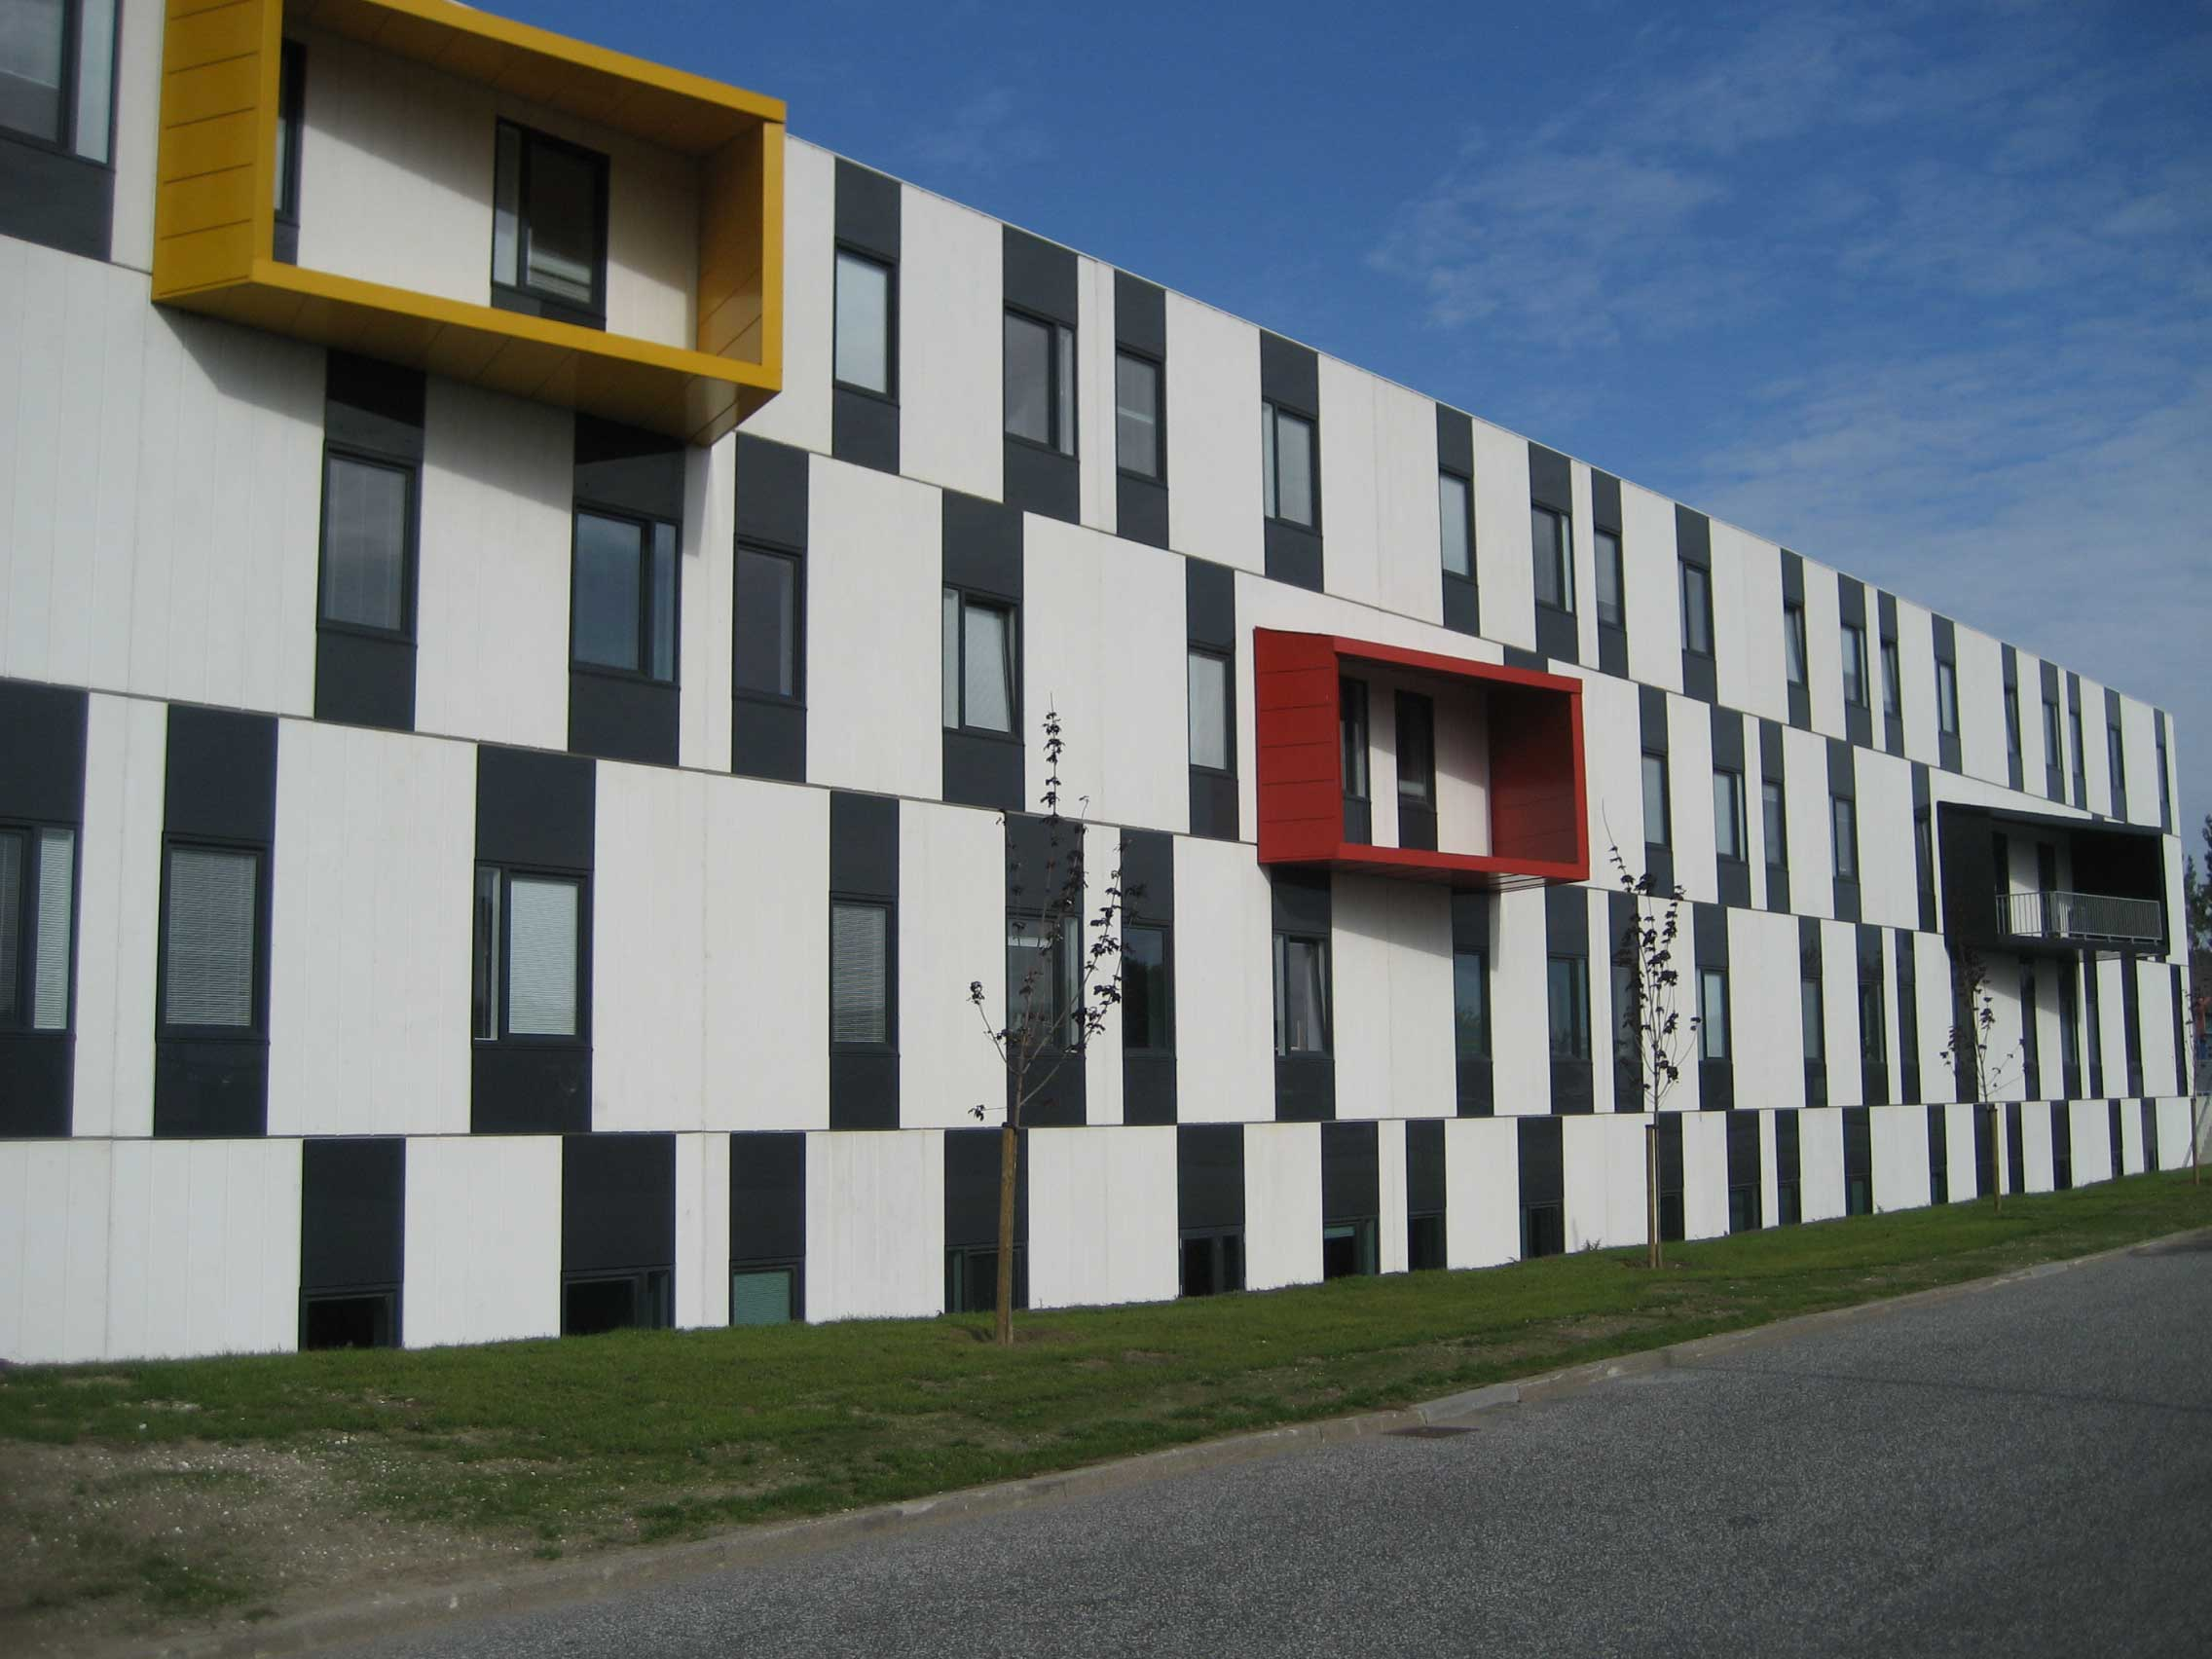
\includegraphics[width=0.9\textwidth]{billeder/forside.jpg}

\vspace{2cm} 
\textsc{\Large P4 Project \\
Group sw408f16 \\
Software\\
Aalborg Universitet\\
Den 26. maj 2016\\}
\end{flushright}

\cleardoublepage												% Indsaetter tom side, saa naeste kapitel starter paa hoejre side (hvis noedvendigt)
% Dette er LaTeX-versionen af titelbladet for TNB studenterrapporter
% Filen kræver:
% Universitetets logo:  AAU-logo-stud-UK eller AAU-logo-stud-DK
% Synopsis: En fil ved navn synopsis.tex

% Udarbejdet af: Jesper Nørgaard (jesper@noergaard.eu) 10. april 2012

\phantomsection
\pdfbookmark[0]{Titelblad}{titelblad}
\thispagestyle{empty}

\begin{minipage}[t]{0.48\textwidth}
\vspace*{-25pt}			%\vspace*{-9pt}

\includegraphics[height=4cm]{billeder/AAU-logo-stud-DK-RGB}
\end{minipage}
\hfill
\begin{minipage}[t]{0.48\textwidth}
{\small 
\textbf{Første Studieår v/ Det Teknisk-}\\
\textbf{Naturvidenskabelige Fakultet}  \\
Byggeri og Anlæg \\
Strandvejen 12-14 \\
9000 Aalborg \\
http://www.tnb.aau.dk}
\end{minipage}

\vspace*{1cm}

\begin{minipage}[t]{0.48\textwidth}
\textbf{Titel:} \\[5pt]\bigskip\hspace{2ex}
Energirenovering

\textbf{Projekt:} \\[5pt]\bigskip\hspace{2ex}
P1-projekt

\textbf{Projektperiode:} \\[5pt]\bigskip\hspace{2ex}
September 2014 - December 2014

\textbf{Projektgruppe:} \\[5pt]\bigskip\hspace{2ex}
B131	

\textbf{Deltagere:} \\[5pt]\hspace*{2ex}
Adam  G. Hansen \\\hspace*{2ex}
Berit Jørgensen \\\hspace*{2ex}
Christoffer Haning \\\hspace*{2ex}
Dorthe Møller \\\hspace*{2ex}
Ejnar V. Jensen \\\hspace*{2ex}
Freja Poulsen \\\bigskip\hspace{2ex}
Gerhard Pedersen

\textbf{Vejledere:} \\[5pt]\hspace*{2ex}
Carsten Henningsen \\\bigskip\hspace{2ex}
Lotte Dalgaard

\vspace*{1cm}

\textbf{Oplagstal: 10} \\
\textbf{Sidetal: 80} \\
\textbf{Appendiks: 3} \\ 
\textbf{Afsluttet 18-12-2014}

\end{minipage}
\hfill
\begin{minipage}[t]{0.483\textwidth}
Synopsis: \\[5pt]
\fbox{\parbox{7cm}{\bigskipSynopsis

\bigskip}}
\end{minipage}

\vfill

{\footnotesize\itshape Rapportens indhold er frit tilgængeligt, men offentliggørelse (med kildeangivelse) må kun ske efter aftale med forfatterne.}

% Rapportens indhold er frit tilgængeligt, men offentliggørelse (med kildeangivelse) må kun ske efter aftale med forfatterne.
% The content of the report is freely available, but publication (with source reference) may only take place in agreement with the authors.

\cleardoublepage
\chapter*{Forord}

Denne rapport er udarbejdet af en gruppe studerende på 1. semester på Byggeri og Anlægs-uddannelsen ved Aalborg Universitet. \textit{Byggeboom i Aalborg} er det overordnede tema for projektet.

Fra projektkataloget er der valgt projektet \textit{Energirenovering}, som lægger op til at belyse andre sider af et byggeboom. Projektet omfatter en kontekstuel vinkel og en teknisk vinkel. Den tekniske del belyser faglighederne energi og indeklima samt konstruktion. Den konstekstuelle del af rapporten behandler ...

Forudsætningerne for at læse rapporten er et vist kendskab til ... \\
Der rettes stor tak til vejlederne ... for inspirerende vejledning og konstruktiv kritik. Endvidere rettes en stor tak til ...

\textbf{Læsevejledning}

Der vil igennem rapporten fremtræde kildehenvisninger, og disse vil være samlet i en kildeliste bagerst i rapporten. Der er i rapporten anvendt kildehenvisning efter Harvardmetoden, så i teksten refereres en kilde med [Efternavn, År]. Denne henvisning fører til kildelisten, hvor bøger er angivet med forfatter, titel, udgave og forlag, mens Internetsider er angivet med forfatter, titel og dato. Figurer og tabeller er nummereret i henhold til kapitel, dvs. den første figur i kapitel 7 har nummer 7.1, den anden, nummer 7.2 osv. Forklarende tekst til figurer og tabeller findes under de givne figurer og tabeller.

\phantom{Luft}

\phantom{Luft}

\begin{table}[H]
	\centering
		\begin{tabular}{c c c}
			\underline{\phantom{mmmmmmmmmmmmmm}} & \underline{\phantom{mmmmmmmmmmmmmm}} & \underline{\phantom{mmmmmmmmmmmmmm}} \\
			Adam  G. Hansen			& Berit Jørgensen 		& Christoffer Haning 			\\
			&&\\
			&&\\
			\underline{\phantom{mmmmmmmmmmmmmm}} & \underline{\phantom{mmmmmmmmmmmmmm}} & \underline{\phantom{mmmmmmmmmmmmmm}} \\
			Dorthe Møller			& Ejnar V. Jensen 		& Freja Poulsen 				\\
			&&\\
			&&\\
		 							& \underline{\phantom{mmmmmmmmmmmmmm}} 	&			\\														
									& Gerhard Pedersen 							& 												
		\end{tabular}
\end{table}
\cleardoublepage

%%%% Indholdsfortegnelse (TOC) %%%%

\phantomsection													% Kunstigt afsnit, som hyperlinks kan 'holde fast i'
\pdfbookmark[0]{Indholdsfortegnelse}{indhold}					% Tildeler en klikbar bookmark til den endelige PDF
\tableofcontents*												% Indholdsfortegnelsen (kaldet ToC) 

%\addtocontents{toc}{\protect\newpage}							% Fremtvinger sideskift i ToC hvis noedvendig (der hvor koden placeres)


\mainmatter														% Hovedindhold - nummereres fra side 1

%%%% Rapportindhold %%%% 										% Rapportindholdet boer IKKE indeholde broedtekst - KUN includede filer!

%% Indledende %%												% Opdel evt. i passende afsnit for overblikkets skyld

\chapter{Introduction}

In Danish high schools all kinds of different languages are available for the students, and the programming languages has found their place as well. For beginners, the syntactic rules, type systems and the nature of the language can be hard to comprehend at first, which is why this report will focus on constructing a language for the high school students. The interest for computer games in the 21st century is bigger than ever \citep{Wankel}, and computer games is a fun and educating approach to learning programming languages. Robocode is a game where the player has to code their own robot, giving every player the opportunity to battle each other’s robots, making it a competition of coding the ‘best’ robot. This is mainly coded in Java, which is an object oriented programming language, and this nature of the language can be hard to understand without having programming experience. There is no popular domain-specific language for Robocode, and therefore the high school students, who is not experienced programmers, may not be likely to code a working robot. This is due to the fact that it requires one to know an object oriented language in advance. 

This is a problem, since Robocode could potentially be a great way of introducing these students for programming languages. If there was a domain-specific language, with more intuitive type systems and good writability, students could easily be introduced for a programming language, and afterwards expand their knowledge gradually on a general purpose programming language. In this report, Robocode will be studied, and the final product should be a domain-specific language for Robocode, compiled to Java.
	
Based on the above mentioned introduction, the project will try to answer the following problem statement:

\textbf{How can a domain-specific language for Robocode simplify the creation of a robot for high school students, with little or no experience to programming?} 
\begin{itemize}
	\item How can the Java type system be simplified?
	\item Which constructs are necessary for programming standard robots in Robocode?
	\item How can an easy to use interface be made for the users?
\end{itemize}
\chapter{Analysis}
\label{chap:Analysis}
The analysis chapter is of purpose to create a basis for the further work with developing a programming language to make the use of Robocode easier for new programmers. This chapter contains a description of Robocode and cover the basics of how to use it. 

Further in the analysis the choice of a parser generator for the project will be discussed. The work of the analysis has the purpose of leading to the next chapter, \ref{chap:LanguageDesign}.

\section{Robocode}
\label{sec:Robocode}
Robocode is an Open Source game project on SourceForge originally started by Mathew A. Nelson in late 2000, who was inspired by RobotBattle from the 1990s. Contributors for the Open Source lead to two new projects, RobocodeNG and Robocode 2006, by Flemming N. Larsen. These two new versions had bug fixes, and new features by the community of Robocode, and in 2006 Flemming merged one of the projects, the Robocode 2006, into an official version 1.1.
The Robocode client was introduced in May 2007, which can be used to create the robots for the game. These robots are usually coded in Java, but in the recent years, C\# and Scala are popular as well. \citep{robocode}

In schools and universities, Robocode is introduced for education and research purposes, as it is intended to be fun and easy to understand the core principles: One robot each, with abilities to drive forward, backwards, turn to the sides, and shoot a gun. These core principles can be vastly expanded to more complicated demands, as the robots universe is bigger than it looks at a first glance. \citep{RoboReadMe}

The way this game works, is by writing code in one of their supported programming languages and then setting it into battle with other people’s robots. There are some sample robots, when the game is downloaded, in order to give the users/players a chance to see how it’s supposed to be written and from there, it’s up to the single individual to make the “best” robot. \citep{MyFirstRobot}

There are held tournaments around the world, where people from around the globe compete. It varies in size, some tournaments are only country based, while others are worldwide, some have leagues and the options are more or less limitless. \citep{rc}

As mentioned before, the Robocode is usually coded in Java, which leads to this report only examining Java samples. This is to prevent any misleading keywords or misinterpretations. The Robocode client comes with a text editor, and the sample robots. In this chapter, some of these sample robots will be examined, and the general setup and main events or methods will be presented.

When creating a new robot in the Robocode text editor, the following methods and events are present:

\begin{lstlisting}[caption={Eksampel of the main loop in Robocode} label=run, xleftmargin=.2\textwidth]
public void run() {
	while(true) {
		//Robots behaviour
	}
}
\end{lstlisting}

This method is the loop for the robot, this loop will determine what the robot does constantly, unless interrupted by an event, which the user can define. The robot behaviour is what the user will code as the AI, along with the robot behaviour in the following code snippets.

\begin{lstlisting}[caption={Eksampel of the onScannedRobot event from Robocode} label=osr, xleftmargin=.2\textwidth]
public void onScannedRobot(ScannedRobotEvent e) {
	//Robots behaviour
}
\end{lstlisting}

The robot’s radar will spot enemies when they get within the vision of the radar, which will raise the onScannedRobot event. This event is used to determine how the robot reacts to spotting an enemy, where the ScannedRobotEvent e is the source for information about the enemy robot spotted.

\begin{lstlisting}[caption={Eksampel of the onHitByBullet event from Robocode} label=ohbb, xleftmargin=.2\textwidth]
public void onHitByBullet(HitByBulletEvent e) {
	//Robots behaviour
}
\end{lstlisting}

When the robot gets hit by another robot’s bullet, the event onHitByBullet will be raised. The robot can then be programmed to act a specific way, change behaviour or carry out a task when the event is raised.

\begin{lstlisting}[caption={Eksampel of the onHitWall event from Robocode} label=ohw, xleftmargin=.2\textwidth]
public void onHitWall(HitWallEvent e) {
	//Robots behaviour
}
\end{lstlisting}

When the robot drives into the wall, the event onHitWall will be raised, and the robot can be programmed to do a specific task when this occurs. 

The above mentioned is only a few of the events that can occur in Robocode. In the while loop, events and functions the user can use many build-in methods from the robot class, which is moving and controlling the robot, controlling the radar and the gun and getting information about the battlefield, the user's robot, other robots and many other things. 


In this section the robocode concept will be described. It will include the different functions the system contains.
  
\subsection{Robot}
The robot is the core of the game. The robot can be coded to act differently in various of encounters. There are some events in Robocode that the users can use to program their strategies. One of the events could be onHitWall which basically tells the user that if the robot hits the wall, then the robot will execute the code matches the event that occurred. The robots also have a gun. The gun is used to damage antagonist robots, in the arena. The robot has a gun, and the possibility to choose different types of bullets. For example, one play could use small and fast bullets, they won’t necessarily hurt very much, but it allows the player to shoot more frequent, compared to larger slower bullets. 

The robot also has a radar. The radar allows the robot to scan for other robots scan and walls. This could once again affect the strategies of the robots.

\subsection{Battlefield}
The battlefield is the arena where the robots will fight each other. It’s also the visible field on screen when the game is running. When coding, the battlefield can be used for different reasons, for example, to get the number of enemies that are alive. A robot might be programmed to act differently if there are less than three robots left. All this depends on the way the player decided to program his robot. Some of the other examples that the battlefield can be queried or could be the field size, time or the current round number. 

\subsection{Energy}
Robots have energy, which is the spendable resource when shooting bullets, it is the ‘health’ of a robot, since being hit by a wall or another robots bullet causes a robot to lose energy. But if one robot hits another one, it regains energy. All robots start at 100 energy at the start of a fight, but can exceed this amount, by hitting other robots to regain energy, without losing it. The amount of energy gained when hitting a robot is (3 * bulletpower), which is three times the power you spend shooting it. By being hit by a bullet, the robot lose (4 * bulletpower), and hitting a wall with an AdvancedRobot extended robot will cause the robot to lose energy as well.

If a robot shoots a bullet which uses the last energy that particular robot has, it will be disabled. A disabled robot will not be able to move or shoot. The last shot that robot took, has a chance to restore the robot, if it hits an enemy and thereby regaining energy.
   
Energy for the robots are both the health and the spendable resource for attacking, which makes every decision of manoeuvring and shooting count.

\subsection{Scoring}
Winning in robocode is not about being the sole survivor, not even in the RoboRumble gamemode, which is the “every man for himself” type of gamemode. It is all about scoring, and there are different methods for scoring points. The various types of scoring are as following:
\begin{itemize}
\item Survival score, every time a robot dies, all remaining robots get 50 points.
\item Last survivor bonus, the last robot alive scores 10 points for every other robot that died before it.
\item Bullet damage, robots scores 1 point for every point of damage that robot deals to other robots.
\item Bullet damage bonus, if a robot kills another robot with a shot, it will gain 20\% of all the damage it did to that robot as points.
Ram damage, any robot that rams another robot gains 2 points for each damage they cause through ramming.
\item Ram damage bonus, every time a robot kills another robot by ramming, it scores an additional 30\% of all the damage it did to that robot as points.
\end{itemize}

When all the above scoring points for all robots in a battle has been added up, the robot with the most points wins the game.


\section{Choice of parser generator}
\label{sec:ParserGenerator}
When choosing a parser generator, one also has to choose a lexer generator, for the lexical analysis. The choice of not building a parser for this project without a generator tool, was due to the fact that the ANTLR4 tool had a build-in lexical analyser, and a plugin for Eclipse/IntelliJ, generating abstract syntax trees while writing the grammar. Other parser generators were discussed before making a final decision, such as CUP, but the lack of lexical analysers and abstract syntax tree builders, and at the same time the ease of installing the ANTLR4 parser generator, stated that the ANTLR4 tool was the choice of generator for this project. For the IntelliJ IDE there was a single plugin the user had to install, but for Eclipse, and the abstract syntax tree builder for Eclipse, it required a few plugins, and a bit of experience with the tool, to fully understand how to operate with the tree builder window. Both Eclipse and IntelliJ has been considered as the IDE to use. IntelliJ is preferred because of the ease of installation and use of the ANTLR4 plugin.
 
\section{ANTLR4 parser generator}
\label{Antlr}
In this project, the ANTLR4 parser generator was chosen, as the tool generated both the parser and the lexical analyzer. This tool, as a plug-in for both IntelliJ and Eclipse, could also build abstract syntax trees (AST), which are the trees representing abstract syntactic structures, language correct (syntactically-correct) sentences (source code) in a computer language. These trees have a top representing the program, and nodes representing terminals and non-terminals. The roots of the tree are terminals, which is the syntactically correct sentence.

The AST tree builder for the ANTLR4 IntelliJ plugin would show the trees in an IntelliJ window, where the user would be able to write a sentence, and the window would show the AST for that particular sentence, if it was syntactically correct, corresponding to the grammar described in a .g4 file in the IntelliJ project.
ANTLR4 parses through an LL(*) algorithm, which means it can process any LL(x) grammar, where ‘x’ is the amount of lookahead needed for parsing, and the LL means it parses from left to right, with leftmost derivation. This makes it a top-down parser. The grammar input to this tool should be a CFG (Context-free grammar) in EBNF (Extended Backus-Naur form), which is a formal description of a formal language, including programming languages. This parser generator can parse to four different languages, where the interesting one for this project would be Java. This tool can also generate a C\# output parser, but as this project narrows Robocode to only be written in Java, this wasn't in consideration for choosing the parser generator. Robocode can, as earlier stated, also be written in C\#, which would enforce the choice made, if this project also included the C\# source code for Robocode.

The ANTLR4 tool for Eclipse required a few other plugins to make the AST window work correctly, and it is a little bugged. When the user defines a grammar, the user then generates an ANTLR4 recognizer, if the .g4 file is then saved, the user then has to edit the document to make it a not-saved file to operate in the AST window. If the user has saved the document, without editing afterwards, the window would be unresponsive.

In IntelliJ the ANTLR4 plugin requires very little work to get started. To generate the ANTLR4 files the user has to right click and select the generate options of the plugin and the IDE does all the work. Similarly to generate the AST all one has to do is right click and choose to test the grammar.


%% Kontekst %%
\chapter{Language design}
\label{chap:LanguageDesign}
In this chapter the design decisions made during the process of creating the language will be described here. There are three criteria for the development of the language, \emph{readability, writability} and \emph{reliability}. The decisions made to accommodate these will be described in detail in the first section of the chapter. 
In the next section, the MoSCoW method and the application of it in the design process will be described. 
 
\section{Language criteria}
\label{sec:LanguageCriteria}
In this section the three main criteria for designing the language will be discussed with focus on the implementation of these in the language. The criteria are based on theory from the book \emph{Concepts of Programming Languages} \citep{Sebesta}. The whole section will be based on this concept.

\subsection{Readability}
Readability is referring to the ease of reading and understanding a programming language. The language in this report should be very simple, since the programming language is, as earlier mentioned, targeted for high school students with little or no programming experience. Therefore the only the necessary features for a beginner in both programming and RoboCode should be implemented. 

Since the language is targeted for beginners, one of the criterias for the language would be to make the syntax as simple as possible, but still have it generally look like Java. The language should also have a high level of orthogonality, which also will help make the language simpler. 

\subsection{Writability}
The general purpose for a DSL language is a language is to be able to make solutions for a specific problem, therefore the writability is important in this project, since the purpose of this project is to make a DSL language for RoboCode. As mentioned in the section above, the language should have a high level of orthogonality, which will also help on  the writability of the language. 
Reliability

\subsection{Reliability}
REMEMBER TO INSERT!

\section{MoSCoW analysis}
\label{sec:MoSCoW}
INTRO

\textbf{Must have}
\begin{itemize}
\item Primitive types and variables (assignment)
\item While loop
\item Reserved calls
\item Robot naming
\item If/Else/Elseif statements)
\item Arithmetic expressions and operators
\item Logical expressions and operators
\end{itemize}
\textbf{Should have}
\begin{itemize}
\item Events
\item Void and type methods
\item Cos, Sin \& Tan
\end{itemize}
\textbf{Could have}
\begin{itemize}
\item For loops
\item Arrays
\item Strings
\item Print statements
\item Comments
\item Setup block
\end{itemize}
\textbf{Want to have, but can’t right now}
\begin{itemize}
\item Random number generator
\item Other robot types
\item Other RoboCode gamemodes
\end{itemize}

 


%% Teknisk %%


%% Afrunding %%

\chapter{Conclusion}


\chapter{Discussion}
\label{chap:Discussion}

Error handling - evt. med en error stack ?
Vi kunne have haft ét symbol table?
Tjekke efter moscow,
Generelt hvad vi har opnået


In section \ref{sec:MoSCoW} the MoSCoW analysis was created and described. The method was used to prioritize the requirements for the project's language. Table \ref{moscowDis} shows which of the requirements that have been implemented and which have not been implemented. \newline
All \textit{Must have} requirements has been implemented as they should, since these were the most important and essential requirements for the language. These were needed to make the logic, movement etc., for the robot. \newline
All \textit{Should have} requirements has also been implemented. The Events and Void and type methods helps the users in order to make more intelligent robots, where Comments are useful for the readability of the program, made by the user. \newline
Most of the requirements in \textit{Could have}, has been implemented, which is Print statements, Strings and Setup block. Print statements and Strings have been implemented for the user to be able to debug their code. The Setup block is used for code, that should only be run once each round. Here the user could write code to make some initializing movements e.g. make the  robot move to the wall. Cos, Sin \& Tan and For loops were not implemented in DatLanguage. \newline
None of the requirements from \textit{Won't have} were implemented in this project.

\begin{table}[H]
\centering
\begin{tabular}{ |l|l|l| }
\hline
\multicolumn{3}{ |c| }{MoSCoW analysis} \\
\hline
& MoSCoW items & Status \\
\hline
\multirow{7}{*}{Must have} & Primitive types and variables & Implemented \\
& While loop & Implemented \\
& Reserved calls & Implemented \\
& Robot naming & Implemented \\
& If/Else/Elseif statements & Implemented \\
& Arithmetic expressions and operators & Implemented \\
& Logical expressions and operators & Implemented \\ \hline
\multirow{3}{*}{Should have} & Events & Implemented \\
& Comments & Implemented \\
& Void and type methods & Implemented \\ \hline
\multirow{6}{*}{Could have} & Cos, Sin \& Tan & {\color{red}Not Implemented} \\
& For loops & {\color{red}Not Implemented} \\
& Print statements & Implemented \\
& Strings & Implemented \\
& Setup block & Implemented  \\ \hline
\multirow{3}{*}{Won't have} & Random number generator & {\color{red}Not Implemented} \\
& Other robot types & {\color{red}Not Implemented} \\
\hline
\end{tabular}
\caption{Fulfilment of the MoSCoW analysis}
\label{moscowDis}

\end{table}
\include{formalia/futurework}

%%%% Kilder %%%%

\begingroup
	\raggedright
	\bibliography{bibtex/litteratur}							% Litteraturlisten inkluderes
\endgroup


%%%% Fixme-listen %%%%

\newpage														% Ny side til Fixme-listen
\listoffixmes													% Fixme-listen - fjernes til sidst i projektet med "%"


%%%% Appendiks %%%%

\appendix														% Appendiks/bilag start - giver chapter bogstaver i stedet for tal
\clearforchapter												% Sikrer at pagestylen aktiveres paa den rigtige side
\phantomsection													% Kunstigt afsnit, som hyperlinks kan 'holde fast i'
\pdfbookmark[0]{Appendiks}{appendiks}							% Tildeler en klikbar bookmark til den endelige PDF

%% Indstillinger for appendiks (deaktiveret med "%") %%

%\pagestyle{empty}												% Sidehoved/-fod for standardsider aendres til tom for appendiks
%\aliaspagestyle{chapter}{empty}								% Sidehoved/-fod for kapitelsider aendres til tom for appendiks
%\settocdepth{chapter}											% Kun kapitel-niveau vises i ToC
%\addtocontents{toc}{\protect\cftpagenumbersoff{chapter}}		% Sidetal for kapitler fjernes i ToC

%% Filer til appendiks %%

\chapter{Appendiks name} \label{sec:ap1}
\begin{center}
    \begin{tabular}{ | l| l | p{0.5\linewidth} | }
    \hline
    Reserved calls & Our language & RoboCode \\ \hline
    Tank. & forward(num distance) & ahead(double distance)  \\ \hline
     & backward(num distance) & back(double distance)  \\ \hline
     & doNothing() & doNothing() \\ \hline
     & energy() & getEnergy() \\ \hline
     & heading() & getHeading() \\ \hline
     & height() & getHeight() \\ \hline
     & width() & getWidth()  \\ \hline
     & velocity() & getVelocity()  \\ \hline
     & xCoord() & getX() \\ \hline
     & yCoord & getY() \\ \hline
     & stop() & stop() \\ \hline
     & resume() & resume() \\ \hline
     & turn(num degrees) & turnLeft(double degrees)  \\ \hline
     & &  \\ \hline
    Gun. & shoot(num power) & fire(double power) \\ \hline
     & coolingRate() & getGunCoolingRate() \\ \hline
     & heading() & getGunHeading() \\ \hline
     & heat() & getGunHeat() \\ \hline
     & turn(num ddegrees) & turnGunLeft(double degrees)  \\ \hline
     & adjustGunForRobotTurn(boolean) & adjustGunForRobotTurn(boolean independant) \\ \hline
     & &  \\ \hline
    Radar. & heading() & getRadarHeading() \\ \hline
     & scan() & scan() \\ \hline
     & adjustRadarForGunTurn(boolean) & adjustRadarForGunTurn(boolean independant)  \\ \hline
     & adjustRadarForRobotTurn(boolean) & adjustRadarForRobotTurn(boolean independant) \\ \hline
     & turn(num degrees) & turnRadarLeft(double degrees) \\ \hline
     & &  \\ \hline
    Battlefield. & height() & getBattleFieldHeight() \\ \hline
     & width() & getBattleFieldWidth() \\ \hline
     & numOfRounds() & getNumRounds() \\ \hline
     & enemies() & getOthers() \\ \hline
     & roundNum() & getRoundNum() \\ \hline
     & time() & getTime()  \\
    \hline
    \end{tabular}
\end{center}

\begin{center}
	\begin{tabular}{ | p{0.3\linewidth} | p{0.3\linewidth} | p{0.3\linewidth} |}
		\hline
		OL / Robocode Event& OL Event Information & Robocode Event Information \\ \hline
		BulletHit / onBulletHit& bulletHeading() & getBullet().getHeading() \\ \hline
		& bulletOwner() & getBullet().getName() \\ \hline
		& bulletPower() & getBullet().getPower() \\ \hline
		& bulletVelocity() & getBullet().getVelocity() \\ \hline
		& bulletVictim() & getBullet().getVictim() \\ \hline
		& bulletXCoord() & getBullet().getX() \\ \hline
		& bulletYCoord() & getBullet().getY() \\ \hline
		& bulletIsActive() & getBullet().isActive() \\ \hline
		& energy() & getEnergy() \\ \hline
		BulletHitBullet / onBulletHitBullet& bulletHeading() & getBullet().getHeading() \\ \hline
		& bulletOwner() & getBullet().getName() \\ \hline
		& bulletPower() & getBullet().getPower() \\ \hline
		& bulletVelocity() & getBullet().getVelocity() \\ \hline
		& bulletVictim() & getBullet().getVictim() \\ \hline
		& bulletXCoord() & getBullet().getX() \\ \hline
		& bulletYCoord() & getBullet().getY() \\ \hline
		& bulletIsActive() & getBullet().isActive() \\ \hline
		& enemyBulletHeading() & getHitBullet().getHeading() \\ \hline
		& enemyBulletOwner() & getHitBullet().getName() \\ \hline
		& enemyBulletPower() & getHitBullet().getPower() \\ \hline
		& enemyBulletVelocity() & getHitBullet().getVelocity() \\ \hline
		& enemyBulletVictim() & getHitBullet().getVictim() \\ \hline
		& enemyBulletXCoord() & getHitBullet().getX() \\ \hline
		& enemyBulletYCoord() & getHitBullet().getY() \\ \hline
		& enemyBulletIsActive() & getHitBullet().isActive() \\ \hline
		HitByBullet / onHitByBullet& bearing() & getBearing() \\ \hline
		& bearingDegrees() & getBearingDegrees \\ \hline
		& bulletHeading() & getBullet().getHeading() \\ \hline
		& bulletOwner() & getBullet().getName() \\ \hline
		& bulletPower() & getBullet().getPower() \\ \hline
		& bulletVelocity() & getBullet().getVelocity() \\ \hline
		& bulletVictim() & getBullet().getVictim() \\ \hline
		& bulletXCoord() & getBullet().getX() \\ \hline
		& bulletYCoord() & getBullet().getY() \\ \hline
		& bulletIsActive() & getBullet().isActive() \\ \hline
		& heading() & getHeading() \\ \hline
		& headingDegrees() & getHeadingDegrees() \\ \hline
		& power() & getPower() \\ \hline
		& velocity() & getVelocity() \\ \hline
		HitRobot / onHitRobot & bearing() & getBearing() \\ \hline
		& bearingDegrees() & getBearingDegrees \\ \hline
		& energy() & getEnergy() \\ \hline
		& myFault() & isMyFault() \\ \hline
		& enemyName() & getName() \\ \hline
		Death / onDeath & & \\ \hline
		HitWall / onHitWall & bearing() & getBearing() \\ \hline
		EnemyDeath / onRobotDeath & enemyName() & getName() \\ \hline
		RoundEnded / onRoundEnded & round() & getRound() \\ \hline
		& totalTurns() & getTotalTurns() \\ \hline
		& turns() & getTurns() \\ \hline
		ScannedRobot / onScannedRobot & bearing() & getBearing() \\ \hline
		& distance() & getDistance() \\ \hline
		& energy() & getEnergy() \\ \hline
		& heading() & getHeading() \\ \hline
		& enemyName() & getName() \\ \hline
		& velocity() & getVelocity() \\ \hline
		Status / onStatus & distanceRemaining() & getStatus.getDistanceRemaining() \\ \hline
		& gunTurnRemaining() & getStatus.getGunTurnRemaining() \\ \hline
		& radarTurnRemaining() & getStatus.getRadarTurnRemaining() \\ \hline
		Win / onWin &  & \\
		\hline
	\end{tabular}
\end{center}


%%%% Bilag %%%%

%\phantomsection												% Kunstigt afsnit, som hyperlinks kan 'holde fast i'
%\addcontentsline{toc}{chapter}{Bilag A \ Navn} 				% Manuelle indgange i indholdsfortegnelsen (naar \includepdf bruges)

%\includepdf[pages={x-y}]{filnavn}								% Inkluder eksterne bilag med \includepdf[pages={x-y}]{filnavn}


\end{document}													% Slutter dokumentet - obligatorisk


